\subsection{Network Interface Controller}
\noindent {\bf Description:}

Module responsible for passing Ethernet frames between the Linux running
on the main ARM processor and 18 ports of WR Switch. It contains a \emph{frame
buffer} and two RAM blocks (\emph{TX descriptors memory}, \emph{RX descriptors
memory}) storing descriptors for frames received and frames to be sent.
Frame buffer stores all frames received from physical ports of WR Switch
(addressed to the main processor) and frames that main processor wants to send
to the ports of WR Switch. Each frame has an associated descriptor which
contains various information about its structure (figure \ref{fig:nic:tx_desc}
and figure \ref{fig:nic:rx_desc}).

When software running on main CPU wants to send an Ethernet frame, it has to
write it to the \emph{frame buffer} and then store the Tx descriptor describing
this frame into \emph{TX descriptors memory}. The other way round, first
software has to write an empty Rx descriptor (\emph{empty} bit set to \emph{1})
into the \emph{RX descriptors memory}. It has to describe the offset and length
of the area in the \emph{frame buffer} where \emph{NIC} can store received
frame. When a new frame is received \emph{NIC} will fill the Rx descriptor and
set \emph{empty} bit to \emph{0}.

When configured, \emph{Network Interface Controller} can also trigger three
different interrupts when:
\begin{itemize}
  \item a new Ethernet frame was received
  \item transmission of the frame is completed
  \item an error has occurred during the frame's transmission
\end{itemize} 
They are all combined into a single IRQ line connected to \emph{Vectored
Interrupt Controller} (sec.\ref{sec:vic}) so wishbone control register has to be
read to get the event which caused the interrupt.

\begin{figure}[ht]
  \begin{center}
    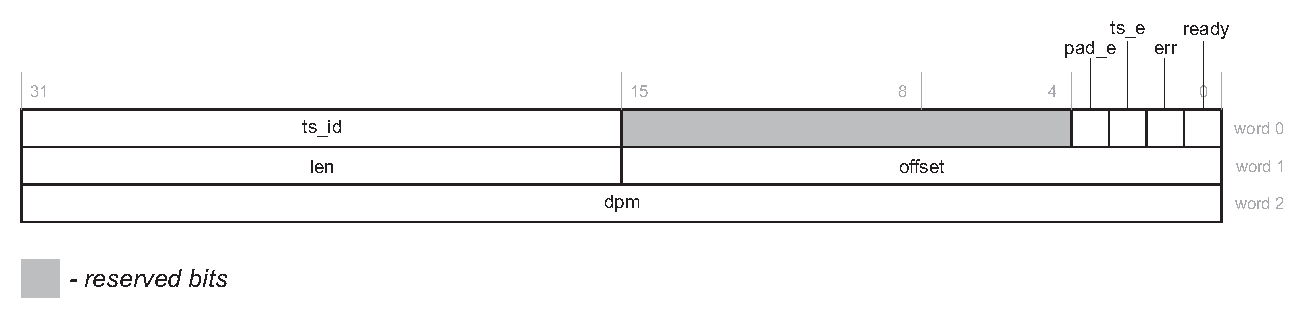
\includegraphics[width=\textwidth]{switch/nic_txdesc.pdf}
    \caption{Tx descriptor}
    \label{fig:nic:tx_desc}
  \end{center}
\end{figure}
\newpage
\begin{tabular}{l p{12cm}}
  \emph{ready} & if \emph{1}, whole descriptor is stored in memory, frame can be
  transmitted\\
  \emph{err} & if \emph{1}, an error has occurred during frame's
    transmission\\
  \emph{ts\_e} & if \emph{1}, request frame timestamping\\
  \emph{pad\_e} & if \emph{1}, frame is runt and requires padding\\
  \emph{ts\_id} & frame id, needed to associate Tx timestamp (from Tx
    Timestamping Unit) with appropriate frame\\
  \emph{offset} & offset of the frame inside \emph{frame buffer}\\
  \emph{len} & length of the frame\\
  \emph{dpm} & destination port mask, each bit set to \emph{1} will
    result in Ethernet frame sent from that physical port\\
\end{tabular}


\begin{figure}[ht]
  \begin{center}
    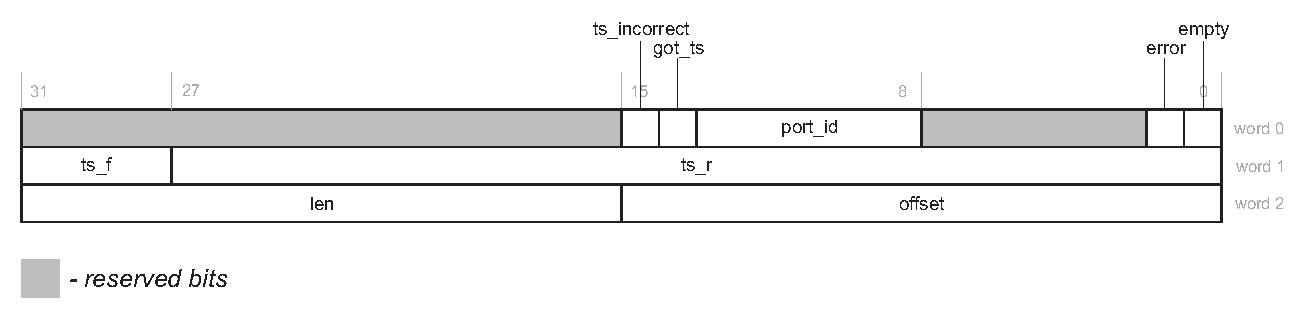
\includegraphics[width=\textwidth]{switch/nic_rxdesc.pdf}
    \caption{Rx descriptor}
    \label{fig:nic:rx_desc}
  \end{center}
\end{figure}
\begin{tabular}{l p{12cm}}
  \emph{empty} & if \emph{1}, descriptor is empty, and can be written by
  reception FSM\\
  \emph{error} & if \emph{1}, an error has occurred during the reception of the
  frame\\
  \emph{port\_id} & the ID of the physical port which has received the frame\\
  \emph{got\_ts} & if \emph{1}, received frame contains OOB data with Rx
  timestamp\\
  \emph{ts\_incorrect} & if \emph{1}, Rx timestamp may be incorrect (generated
  during the adjustment of time base)\\
  \emph{ts\_r} & Rx timestamp generated on the rising edge of the reference
  clock\\
  \emph{ts\_f} & least significant bits of the Rx timestamp generated on the
  falling edge of the reference clock\\
  \emph{offset} & offset of the frame inside \emph{frame buffer}\\
  \emph{len} & length of the allocated buffer for Rx frame (when \emph{empty}
  is \emph{1}) or length of the received frame (when \emph{empty} is \emph{0})
  received frame when
\end{tabular}

\vspace{12pt}
\noindent{\bf Wishbone interface:}

Wishbone interface of WR NIC contains two areas with different base addresses:\\

\begin{tabular}{l l}
  configuration registers & 0x20000\\
            frame buffer  & 0x28000\\
\end{tabular}

\vspace{12pt}
The description of configuration registers can be found in section
\ref{subsec:wbgen:nic}.
